\documentclass[border=10pt]{standalone}
\usepackage{pgfplots}
\pgfplotsset{compat=1.18}
\begin{document}
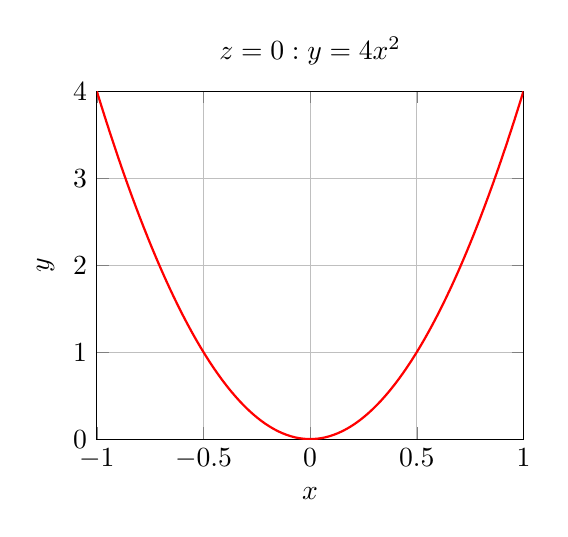
\begin{tikzpicture}
\begin{axis}[
    width=7cm, height=6cm,
    xlabel=$x$, ylabel=$y$,
    xmin=-1, xmax=1,
    ymin=0, ymax=4,
    grid=major,
    title={$z=0: y=4x^2$}
]
\addplot[red, thick, domain=-1:1, samples=100] {4*x^2};
\end{axis}
\end{tikzpicture}
\hspace{1cm}
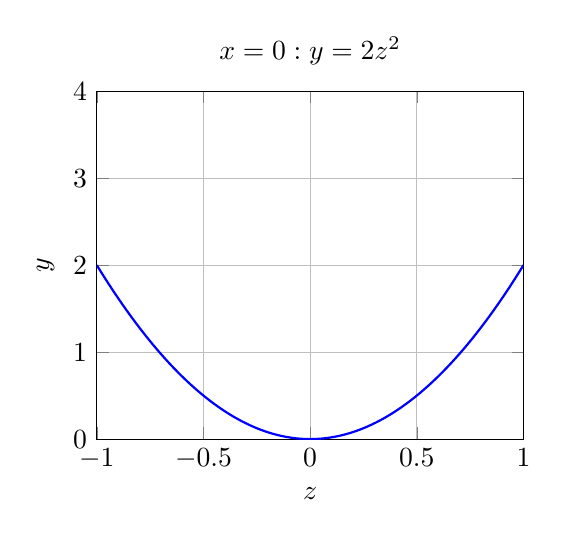
\begin{tikzpicture}
\begin{axis}[
    width=7cm, height=6cm,
    xlabel=$z$, ylabel=$y$,
    xmin=-1, xmax=1,
    ymin=0, ymax=4,
    grid=major,
    title={$x=0: y=2z^2$}
]
\addplot[blue, thick, domain=-1:1, samples=100] {2*x^2};
\end{axis}
\end{tikzpicture}
\end{document}
